% Copyright (c) 2015 William Bevington, Callum O'Brien and Alex Pace

% Permission is granted to copy, distribute and/or modify this document
% under the terms of the GNU Free Documentation License, Version 1.3
% or any later version published by the Free Software Foundation;
% with no Invariant Sections, no Front-Cover Texts, and no Back-Cover Texts.

\documentclass{article}

\usepackage{amsmath}
\usepackage{amssymb}

\usepackage{array}

\usepackage{geometry}

\usepackage{mathrsfs}

\usepackage{multicol}

\usepackage{tikz}
\usetikzlibrary{arrows}

\newcommand{\de}{\textrm{d}\,}
\newcommand{\st}{\:|\:}
\newcommand{\csch}{\textrm{csch\,}}
\newcommand{\sech}{\textrm{sech\,}}
\newcommand{\arsinh}{\textrm{arsinh\,}}
\newcommand{\arcosh}{\textrm{arcosh\,}}
\newcommand{\artanh}{\textrm{artanh\,}}

\begin{document}

\title{FP3}
\author{William Bevington \and Callum O'Brien \and Alex Pace}
\maketitle
\tableofcontents
\newpage

\section{Hyperbolic Functions}

The hyperbolic functions are analogs of the ordinary trigonometric, or circular
functions. The basic hyperbolic functions are, as one might expect, analygous to
sine and cosine; they are hyperbolic sine and hyperbolic cosine.\\
The following graphs plot the various hyperbolic trigonometric functions, allong the left hand side is the hyperbolic function of sin and its counterparts, down the middle hyperbolic cos, and the right hyperbolic tan. The domain and range of each function is also described below their respective graphs.

\begin{center}
    
    \begin{tikzpicture}[xscale=0.5,yscale=0.25]
    
        \draw[<->] (-3,0) -- (3,0);
        \draw[<->] (0,6) -- (0,-6);
    
        \draw[cyan,domain=-2.4:2.4] plot (\x, {sinh(\x)});

    \end{tikzpicture} \hspace{50pt} \begin{tikzpicture}[xscale=0.5,yscale=0.25]
    
        \draw[<->] (-3,0) -- (3,0);
        \draw[<->] (0,6) -- (0,-6);

        \draw[cyan,domain=-2.4:2.4] plot (\x, {cosh(\x)});

    \end{tikzpicture} \hspace{50pt} \begin{tikzpicture}[xscale=0.5,yscale=0.25]
    
        \draw[<->] (-3,0) -- (3,0);
        \draw[<->] (0,6) -- (0,-6);
    
        \draw[cyan,domain=-2.4:2.4] plot (\x, {tanh(\x)});

    \end{tikzpicture}

\end{center}

\hspace{5pt} \begin{tabular}{lll}
    
    \(\sinh(x)\) \hspace{100pt} & \(\cosh(x)\) \hspace{100pt} & \(\tanh(x)\) \\
    
    \textbf{Domain} \(\left\{x\in\mathbb{R}\right\}\) & \textbf{Domain} \(\left\{x\in\mathbb{R}\right\}\) & \textbf{Domain} \(\left\{x\in\mathbb{R}\right\}\) \\
    
    \textbf{Range} \(\left\{y\in\mathbb{R}\right\}\) & \textbf{Range} \(\left\{y\in\mathbb{R}\,|\,y\geq1\right\}\) & \textbf{Range} \(\left\{y\in\mathbb{R}\,|\,-1<y<1\right\}\)

\end{tabular}

\begin{center}
    
    \begin{tikzpicture}[xscale=0.5,yscale=0.25]
            
        \draw[<->] (-3,0) -- (3,0);
        \draw[<->] (0,6) -- (0,-6);
        
        \draw[cyan,domain=-2.4:-0.2] plot (\x, {1/sinh(\x)});
        \draw[cyan,domain=0.2:2.4] plot (\x, {1/sinh(\x)});
    
    \end{tikzpicture} \hspace{50pt} \begin{tikzpicture}[xscale=0.5,yscale=0.25]
        
        \draw[<->] (-3,0) -- (3,0);
        \draw[<->] (0,6) -- (0,-6);
        
        \draw[cyan,domain=-2.4:2.4] plot (\x, {1/cosh(\x)});
    
    \end{tikzpicture} \hspace{50pt} \begin{tikzpicture}[xscale=0.5,yscale=0.25]
        
        \draw[<->] (-3,0) -- (3,0);
        \draw[<->] (0,6) -- (0,-6);
        
        \draw[cyan,domain=-2.4:-0.2] plot (\x, {1/tanh(\x)});
        \draw[cyan,domain=0.2:2.4] plot (\x, {1/tanh(\x)});
    
    \end{tikzpicture}

\end{center}

\hspace{5pt} \begin{tabular}{lll}
    
    \textrm{csch(x)} \hspace{100pt} & \textrm{sech(x)} \hspace{100pt} & \textrm{coth(x)} \\
    
    \textbf{Domain} \(\left\{x\in\mathbb{R}\,|\,x\neq0\right\}\) & \textbf{Domain} \(\left\{x\in\mathbb{R}\right\}\) & \textbf{Domain} \(\left\{x\in\mathbb{R}\,|\,x\neq0\right\}\) \\
    
    \textbf{Range} \(\left\{y\in\mathbb{R}\,|\,y\neq0\right\}\) & \textbf{Range} \(\left\{y\in\mathbb{R}\,|\,0<y<1\right\}\) & \textbf{Range} \(\left\{y\in\mathbb{R}\,|\,y<-1\textrm{ or }y>1\right\}\)

\end{tabular}

\begin{center}
    
    \begin{tikzpicture}[xscale=0.5,yscale=0.25]
        
        \draw[<->] (-3,0) -- (3,0);
        \draw[<->] (0,6) -- (0,-6);
        
        \draw[cyan,domain=-2.4:2.4] plot (\x, {ln(\x+sqrt(1+\x*\x))});
    
    \end{tikzpicture} \hspace{50pt} \begin{tikzpicture}[xscale=0.5,yscale=0.25]
        
        \draw[<->] (-3,0) -- (3,0);
        \draw[<->] (0,6) -- (0,-6);
        
        \draw[cyan,domain=1:2.4] plot (\x, {ln(\x+sqrt(\x+1)*sqrt(\x-1))});
    
    \end{tikzpicture} \hspace{50pt} \begin{tikzpicture}[xscale=0.5,yscale=0.25]
        
        \draw[<->] (-3,0) -- (3,0);
        \draw[<->] (0,6) -- (0,-6);
        
        \draw[cyan,domain=-0.99999:0.99999] plot (\x, {0.5*(ln(1+\x)-ln(1-\x))});
    
    \end{tikzpicture}

\end{center}

\hspace{5pt} \begin{tabular}{lll}
    
    \(\sinh^{-1}(x)\) \hspace{85pt} & \(\cosh^{-1}(x)\) \hspace{85pt} & \(\tanh^{-1}(x)\) \\
    
    \textbf{Domain} \(\left\{x\in\mathbb{R}\right\}\) & \textbf{Domain} \(\left\{x\in\mathbb{R}\,|\,x\geq1\right\}\) & \textbf{Domain} \(\left\{x\in\mathbb{R}\,|\,-1<x<1\right\}\) \\
    
    \textbf{Range} \(\left\{y\in\mathbb{R}\right\}\) & \textbf{Range} \(\left\{y\in\mathbb{R}\right\}\) & \textbf{Range} \(\left\{y\in\mathbb{R}\right\}\)

\end{tabular}

\subsection{Inverse Hyperbolic Trigonometric Functions}

The inverse of a hyperbolic function reverses the operation of the corresponding trigonometric function. Therefore, these functions can be used to find a certain input of a hyperbolic trigonometric function haven being given its output.

\[\textrm{arsinh}\left(z\right)=\ln\left(z+\sqrt{1+z^2}\right)\]

\noindent this identity can be found through the following process:

\[z=\sinh\left(x\right)\]
\[z=\frac{e^x-e^{-x}}{2} \: \rightarrow \: 2z=e^x-e^{-x}\]
\[2ze^x=e^{2x}-1 \: \rightarrow \: \left(e^x\right)^2-2z\left(e^x\right)-1=0\]

\noindent This should be recognizable as a quadratic equation with \(e^x\) instead of the regular \textrm{x}, the variable \textrm{z} will be considered a constant. \\
Using the quadratic formula, you should obtain:

\[e^x=z\pm\sqrt{z^2+1}\]

\noindent At this point you should realise that \(e^x\,>\,0\) for all \textrm{x}, and considering \(\sqrt{z^2+1}\,>\, y\), we can discard the solution with the minus sign and then take the natural logarithm of both sides to arrive at our solution for \textrm{x}:

\[e^x=z+\sqrt{z^2+1} \: \rightarrow \: x=\ln\left(z+\sqrt{z^2+1}\right)\]

\noindent similarly, the inverse of \(\cosh\left(x\right)\) is defined thus:

\[\textrm{arcosh}\left(z\right)=\ln\left(z+\sqrt{z+1}\sqrt{z-1}\right)\]

\noindent It is also derived in a similar fashion:

\[z=\cosh\left(x\right)\]
\[z=\frac{e^x+e^{-x}}{2} \: \rightarrow \: 2z=e^x+e^{-x}\]
\[2ze^x=e^{2x}+1 \: \rightarrow \: \left(e^x\right)^2-2z\left(e^x\right)+1=0\]

\noindent again this is a quadratic equation which can be solved to find the following:

\[e^x=z\pm\sqrt{z^2-1}\]

\noindent since \(x\geq0\) we know that \(e^x\geq1\) for all \textrm{x}. And since \(z-\sqrt{z^2-1}\) does not exceed \(1\) for some \textrm{y}, we must discard the solution with the minus sign. This leaves us with a difference of two squares which can be sepearted to find all solutions of \textrm{x}.

\[e^x=z+\sqrt{z^2-1} \: \rightarrow \: e^x=z+\sqrt{z+1}\sqrt{z-1}\]

\[x=\ln\left(e^x=z+\sqrt{z+1}\sqrt{z-1}\right)\]

\noindent finally, inverse \(\tanh\left(x\right)\) is defined:

\[\textrm{artanh}\left(z\right)=\frac{1}{2}\left(\ln\left(1+z\right)-\ln\left(1-z\right)\right)\]

\noindent and is derived:

\[z=\tanh\left(x\right)\]
\[z=\frac{e^x-e^{-x}}{e^x+e^{-x}}=\frac{e^{2x}-1}{e^{2x}+1}\]
\[\left(e^{2x}+1\right)z=e^{2x}-1 \: \rightarrow \: \left(z-1\right)e^{2x}+z+1=0\]

\noindent solving this quadratic equation yields:

\[e^x=\pm\sqrt{\frac{z+1}{1-z}}\]

\noindent because \(e^x>0\) we must disregard the negative solution. Then from here we can take the natural logarithm of both sides and simplify to find our solution:

\[e^x=\sqrt{\frac{z+1}{1-z}} \: \rightarrow \: x=\ln\left(\sqrt{\frac{z+1}{1-z}}\right)\]

\[x=\frac{1}{2}\ln\left(\frac{z+1}{1-z}\right) \: \rightarrow \: x=\frac{1}{2}\left(\ln\left(1+z\right)-\ln\left(1-z\right)\right)\]


\section{Conic Sections}

\begin{center}
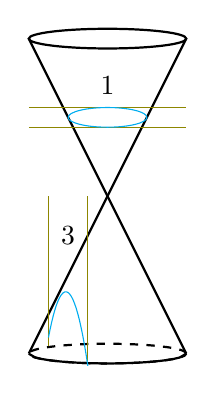
\begin{tikzpicture}[xscale=0.5,yscale=0.5]
    \draw[thick, domain=-2:2] plot (\x, {2*\x});
    \draw[thick, domain=-2:2] plot (\x, {-2*\x});
    \draw[thick] (0,4) ellipse (2 and 1/4);
    \draw[thick, domain=2:-2] plot (\x, {0.125*(-sqrt(4-(\x*\x))-32)});
    \draw[thick, dashed] (0,-4) ellipse (2 and 1/4);
    \draw[olive] (-2,1.75) -- (2,1.75);
    \draw[olive] (-2,2.25) -- (2,2.25);
    \draw[cyan] (0,2) ellipse (1 and 1/4);
    \node at (0,2.8) {1};
    \draw[olive] (-1.5,-3.8) -- (-1.5,0);
    \draw[olive] (-0.5,-4.2) -- (-0.5,0);
    \draw[cyan, domain=-1.5:-0.5] plot (\x, {-6*((\x+1.06)*(\x+1.06))-2.43});
    \node at (-1,-1) {3};
\end{tikzpicture} \hspace{50pt} 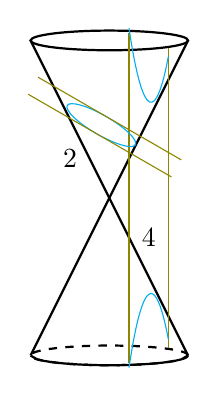
\begin{tikzpicture}[xscale=0.5,yscale=0.5]
    \draw[thick, domain=-2:2] plot (\x, {2*\x});
    \draw[thick, domain=-2:2] plot (\x, {-2*\x});
    \draw[thick] (0,4) ellipse (2 and 1/4);
    \draw[thick, domain=2:-2] plot (\x, {0.125*(-sqrt(4-(\x*\x))-32)});
    \draw[thick, dashed] (0,-4) ellipse (2 and 1/4);
    \draw[olive] (1.5,-3.8) -- (1.5,3.8);
    \draw[olive] (0.5,-4.2) -- (0.5,4.2);
    \draw[cyan, domain=1.5:0.5] plot (\x, {-6*((\x-1.06)*(\x-1.06))-2.43});
    \draw[cyan, domain=1.5:0.5] plot (\x, {6*((\x-1.06)*(\x-1.06))+2.43});
    \node at (1,-1) {4};
    \draw[cyan, rotate=330] (-1.1,1.5) ellipse (1 and 1/4);
    \draw[olive, rotate=330] (-3.1,1.75) -- (1.1,1.75);
    \draw[olive, rotate=330] (-3.1,1.25) -- (1.1,1.25);
    \node at (-1,1) {2};
\end{tikzpicture}
\end{center}

\begin{center}
\begin{tabular}{cccc}
1. Circle & 2. Ellipse & 3. Parabola & 4. Hyperbola \\
\end{tabular}
\end{center}

All conic sections can be described in terms of loci; for any point $P$ on a
conic section,

\[\frac{|PM|}{|PS|} = e\]

\noindent where $e$ is the eccentricity, $S$ is the focus and $M$ is the closest point to
$P$ that lies on the directrix.

\[0 \leq e < 1 \Rightarrow P \textrm{ describes an ellipse}\]
\[e = 1 \Rightarrow P \textrm{ describes a parabola}\]
\[e > 1 \Rightarrow P \textrm{ describes a hyperbola}\]

\begin{multicols}{2}

\vspace{20pt}

\begin{center}

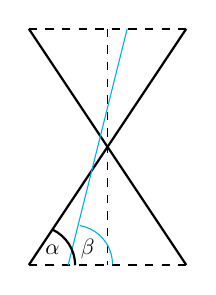
\begin{tikzpicture}[xscale=0.5,yscale=0.5]
    \draw[thick] (-2,-3) -- (2,3);
    \draw[thick] (-2,3) -- (2,-3);
    \draw[thick, dashed] (-2,-3) -- (2,-3);
    \draw[thick, dashed] (-2,3) -- (2,3);
    \draw[dashed] (0,3) -- (0,-3);
    \draw[cyan] (-1,-3) -- (0.5,3);
    \draw[cyan] (-0.7,-2) arc (80:0:1);
    \draw[thick] (-1.4,-2.1) arc (65:0:1);
    \node[scale=0.8] at (-1.4,-2.6) {\(\alpha\)};
    \node[scale=0.8] at (-0.5,-2.6) {\(\beta\)};
\end{tikzpicture}
\end{center}

\noindent The eccentricity can also be defined graphically, in terms of the cone and the intersection. Where \(e\) is the ratio between the angle of the cone and the intersection

\[e=\frac{\sin\left(\beta\right)}{\sin\left(\alpha\right)}\]

\end{multicols}


\subsection{Ellipses}

Ellipses are conic sections with eccentricty $e \in [0,1)$. Considering their
geometry, it is clear that, when expressed as a parametric equation, ellipses
take the form;

\[x = a\cos\theta,\: y = b\sin\theta\]

\noindent Hence;

\[\left(\frac{x}{a}\right)^2 = \cos^2\theta,\: \left(\frac{y}{b}\right)^2 =
\sin^2\theta\]

\noindent Making apparent an ellipse expressed in cartesian form;

\[\left(\frac{x}{a}\right)^2 + \left(\frac{y}{b}\right)^2 = 1\]

\paragraph{Theorem} For $e \in [0,1)$, an ellipse of focus $(ae, 0)$ and
directrix $x = \frac{a}{e}$ is described by the equation;

\[\left(\frac{x}{a}\right)^2 + \left(\frac{y}{b}\right)^2 = 1\]

\paragraph{Proof} 

\[\frac{|PS|^2}{|PM|^2} = e \Rightarrow |PS|^2 = e^2|PM|^2\]

\noindent By pythagoras,

\[|PS|^2 = \left(x - ae\right)^2 + y^2\]

\[|PM|^2 = \left(\frac{a}{e} - x\right)^2 + y^2\]

\noindent Thus

\[\left(x - ae\right)^2 + y^2 = \left(\frac{a}{e} - x\right)^2e^2\]\\

\noindent The derivative of an ellipse can be found by implicitly
differentiating its cartesian form or using the chain rule on its parametric
form. By the former method;

\[\frac{\de}{\de x} \left(\left(\frac{x}{a}\right)^2 +
\left(\frac{y}{b}\right)^2\right) = \frac{\de}{\de x}1\]

\[\frac{2x}{a^2} + \frac{2y}{b^2} \times \frac{\de y}{\de x} = 0\]

\[\frac{\de y}{\de x} = -\frac{b^2x}{a^2y}\]

\noindent And by the latter;

\[\frac{\de x}{\de \theta} = -a\sin\theta\]

\[\frac{\de y}{\de \theta} = b\cos\theta\]

\[\frac{\de y}{\de x} = \frac{\de y}{\de \theta} \times \left(\frac{\de x}{\de
\theta}\right)^{-1} = -\frac{b\cos\theta}{a\sin\theta}\]

\noindent From this we can derive the general equation of a tangent to an
ellipse at a point $\left(i,\, j\right)$:

\[y - j = -\frac{b^2i}{a^2j}\left(x - i\right)\]

\[a^2jy + b^2ix = \left(aj\right)^2 + \left(bi\right)^2\]

\noindent Similarly, we can derive the equation for a normal:

\[y - j = \frac{a^2j}{b^2i}\left(x - i\right)\]

\[b^2iy + a^2ij = a^2jx + b^2ij\]

\subsection{Hyperbolae}

A hyperbola is a conic section with $e > 1$.

\end{document}

